%2025 - 3b
\section{03b Chapitre 2 : Variétés différentielles (fin)}

Fonctions différentiables, C\_k, lisses (C\_infini):

-de R dans M (courbes lisses)

-entre deux variétés différentielles

\subsection{Difféomorphisme}
\[
(M,\ \mc{O}_M,\ \mc{A}_{\infty M})\ \xrightarrow{f}\ (N,\ \mc{O}_N,\ \mc{A}_{\infty N})
\]
Si f continue et différentiable, bijective et $f^{-1}$ continue, différentiable et bijective,

Par définition


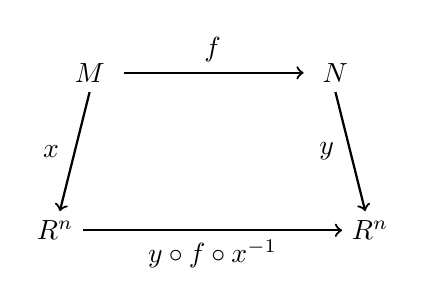
\begin{tikzpicture}
\def\largeur{3} \def\hauteur{2} \def\decalage{0.3} \def\trapeze{0.5}
\node (A) at (0,0) {$M\ $};
\node (B) at (\largeur,0) {$\ N$};
\node (C) at (-\trapeze,-\hauteur) {$\mb{R}^n$};
\node (D) at (\largeur+\trapeze,-\hauteur) {$\mb{R}^n$};
%
\node (I) at (0.5*\largeur ,\decalage) {$f$};
\node (G) at (-0.5*\trapeze-\decalage ,-0.5*\hauteur) {$x$};
\node (H) at (\largeur+0.5*\trapeze-\decalage ,-0.5*\hauteur) {$y$};
\node (E) at (0.5*\largeur ,-\hauteur-\decalage) {$y\circ f\circ x^{-1}$};
\draw[thick,->] (A)--(B);
\draw[thick,->] (A)--(C);
\draw[thick,->] (B)--(D);
\draw[thick,->] (C)--(D);
\end{tikzpicture}

En dimension 1, 2 ou 3, à une variété topologique correspond une seule structure différentielle

En dimension supérieur à 4, il existe un nommbre fini de structure différentielle

En dimension supérieur à 4, il existe une infinité non dénombrable de structure différentielle

\[
\begin{array}{ l c l l }
 \mr{V}_{\gamma,p} : & \mc{C}^\infty(M) & \to & \mb{R} \\ 
  & f & \mapsto & {v}_{\gamma,p}(f)=(f\circ\gamma)'|_{\lambda_0} \\
\end{array}
\]
\[
 \mc{A} = \{ (\mc{U}, x) : \mc{U} \to \mb{R}^n\}
\]
Unicité ou non des structures différentielles (à difféomorphisme près)


